\documentclass[a4paper, 12pt]{article}
\usepackage[usenames,dvipsnames]{xcolor}
\usepackage{fullpage}
\usepackage[top=0.5in, bottom=1in, left=1in, right=1in]{geometry}
\usepackage{amsmath}
\usepackage{fancyhdr}
\usepackage{pgfornament}
\usepackage{multicol}
\usepackage{enumitem}
\usepackage{xspace}
\usepackage{lastpage}
\usepackage{hyperref}
\usepackage{tikz}
\usepackage{tkz-euclide}
\usepackage{pgfplots}
\usepackage{commath}
\usetkzobj{all}
\usepackage{lastpage}
\usepackage{amsfonts}
\usepackage{standalone}
\usetikzlibrary{shapes.misc, angles, quotes, graphs, graphdrawing}
\usegdlibrary{force, layered}



%opening

\newcommand{\epv}[1]{\ensuremath{\left< #1 \right>}\xspace}
\newcommand{\variance}{\ensuremath{\text{Var}}}
\newcommand{\unit}[1]{\;\ensuremath{\mathrm{#1}}\xspace}
\newcommand{\umss}{\;\unit{m/s^2}}
\newcommand{\ums}{\;\unit{m/s}}
\newcommand{\us}{\;\unit{s}}
\newcommand{\um}{\;\unit{m}}
\newcommand{\kwd}[1]{\textbf{\textcolor{Brown}{#1}}}
\pagestyle{fancyplain}
\renewcommand{\headrulewidth}{0pt}
\cfoot{\pgfornament[height=1em, ydelta=-0.4em]{11} \thepage of \pageref{LastPage}  \;\pgfornament[height=1em, ydelta=-0.4em]{14}}
\newenvironment{question}{\begin{minipage}{\linewidth}}{\end{minipage}}
\rhead{Name: \underline{\hspace{7cm}} }
\lhead{ID: \underline{\hspace{4cm}} }
\headheight 15pt              %% put this outside
\headsep 10pt                 %% put this outside
\newcommand{\sanswer}{\vspace{1.25in}}
\newcommand{\manswer}{\vspace{2.5in}}
\newcommand{\lanswer}{\vspace{5in}}
\newcommand{\ssanswer}{\vspace{0.5in}}
\newcommand{\ihat}{\hat{i}}
\newcommand{\jhat}{\hat{j}}
\newcommand{\khat}{\hat{k}}
\newcommand{\hint}{\textbf{Hint:} }
\newcommand{\E}{\mathbb{E}}
\newcommand\NoIndent[1]{%
	\begingroup
	\par
	\parshape0
	#1\par
	\endgroup
}

\pgfplotsset{
	answeraxis/.style={width=6in, height = 3in, grid=both, axis lines=middle, minor tick num=1,  axis line style={very thick, gray!50!white}}
}

\begin{document}
\begin{center}
	\textcolor{orange}{\textsc{Discrete Mathematics}}\\
	\huge\textbf{\textsc{Final Exam T3 2021}}\\
	\pgfornament[width=0.7\textwidth, color=white!30!black]{89}
\end{center}

\textbf{Instruction}
\begin{itemize}
\item Write your name
\item This exam is take home based on your honor code. Open book open notes. But do not communicate with another human being via any means regarding exam. The violations includes but not limited to asking questions on stack overflow, chegg or similar services, or asking your friends via online or offline channel.
\item Read the questions carefully.
\item There are 4 problems. 520 points in total. You only need to get 460 points to get full score.
\item Attempt all problems, state your reasons \emph{clearly} and \emph{legibly}, because partial credits will be given.
\end{itemize}
\vspace{0.25in}

	\begin{center}
		\def\arraystretch{1.5}
		\begin{tabular}{|c|c|c|}
			\hline Question & Full Score & Your Score  \\ 
			\hline  1 & 100 &  \\ 
			\hline  2 & 120 &  \\ 
			\hline  3 & 160 &  \\
			\hline  4 & 140 & \\
			\hline 
		\end{tabular} 
	\end{center}
	

	\def\arraystretch{1.0}


\begin{center}
Total:\; \fbox{ \begin{minipage}{1in} \hfill\vspace{1in} \end{minipage} }/460
\end{center}
\pagebreak
\section*{Useful Formulas}
%\subsection*{Asymptotics}
%\renewcommand{\arraystretch}{2}
%\begin{center}
%	\begin{tabular}{c |c c c | c}
%		\hline\hline
%		Definiton & Definition & & & Intuition\\
%		\hline\hline  Asym. Equal & $f \sim g$ & iff & $\lim\limits_{x\to \infty} \frac{f(x)}{g(x)} = 1$  & $f \underbrace{\equiv}_{x \to \infty} g$\\ 
%		Big Oh & $f \in O(g)$ & iff & $\lim\limits_{x\to \infty} \frac{f(x)}{g(x)} < \infty$ & $f \underbrace{\le}_{x \to \infty} g$  \\ 
%		Little Oh  & $f \in o(g)$ & iff & $\lim\limits_{x\to \infty} \frac{f(x)}{g(x)} = 0$ & $f \underbrace{<}_{x \to \infty} g$ \\ 
%		Little Omega & $f \in \omega(g)$ & iff & $\lim\limits_{x\to \infty} \frac{f(x)}{g(x)} \to \infty$ & $f \underbrace{>}_{x \to \infty} g$ \\ 
%		Big Omega  & $f \in \Omega(g)$ & iff & $\lim\limits_{x\to \infty} \frac{f(x)}{g(x)} > 0 $ & $f \underbrace{\ge}_{x \to \infty} g$ \\ 
%		Theta & $f \in \Theta(g)$ & iff & $\lim\limits_{x\to \infty} \frac{f(x)}{g(x)} =c, c\ne 0$ & $f \underbrace{=}_{x \to \infty} g$ \\ 
%		\hline\hline 
%	\end{tabular}
%\end{center}
\subsection*{Sum}
\begin{align*}
	1 + 2 + 3 + \ldots + n &= \frac{n(n+1)}{2}\\
	1^2 + 2^2 + 3^2 + \ldots + n^2 &= \frac{n(n+1)(2n+1)}{6}\\
	1^3 + 2^3 + 3^3 + \ldots + n^3 &= \left(\frac{n(n+1)}{2}\right)^2\\
	1+3 + 5 + 7 + \ldots + (2n-1) &= n^2
\end{align*}

\subsection*{Euler's Formula}
\[
e+2 = v+f
\]

%\subsection*{Integral}
%\begin{align*}
%	\int x^n \; dx &= \frac{1}{n+1} x^{n+1} &\text{if } n \ne -1\\
%	\int \frac{1}{x} \; dx &= \ln (x)
%\end{align*}


%\subsection*{Quadratic}
%\begin{align*}
%	x = \frac{-b \pm \sqrt{b^2 - 4ac}}{2a}
%\end{align*}

\pagebreak

\begin{enumerate}
	\item Graph Theory(100 points. 20 each)
	\begin{enumerate}
		\item Drawing Graph
		Draw a \textbf{tree} with exacty 5 edges and exactly 3 leaves.
		\sanswer
		\item Find an Euler walk for the following graph. Label the edges with \emph{numbers} so I can follow.	
			\begin{center}
			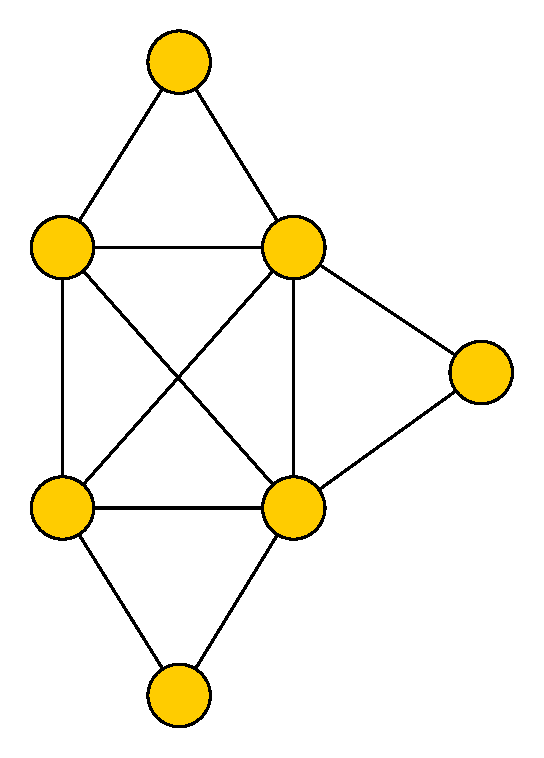
\includegraphics[width=0.5\linewidth]{eulertour}
			\end{center}
		\newpage
		\item The following graph shows the cost of electric wire to connect one city to another(in millions). If your job is to connect every city to electricity grid at the lowest cost, how much money do you need?
			\begin{center}
			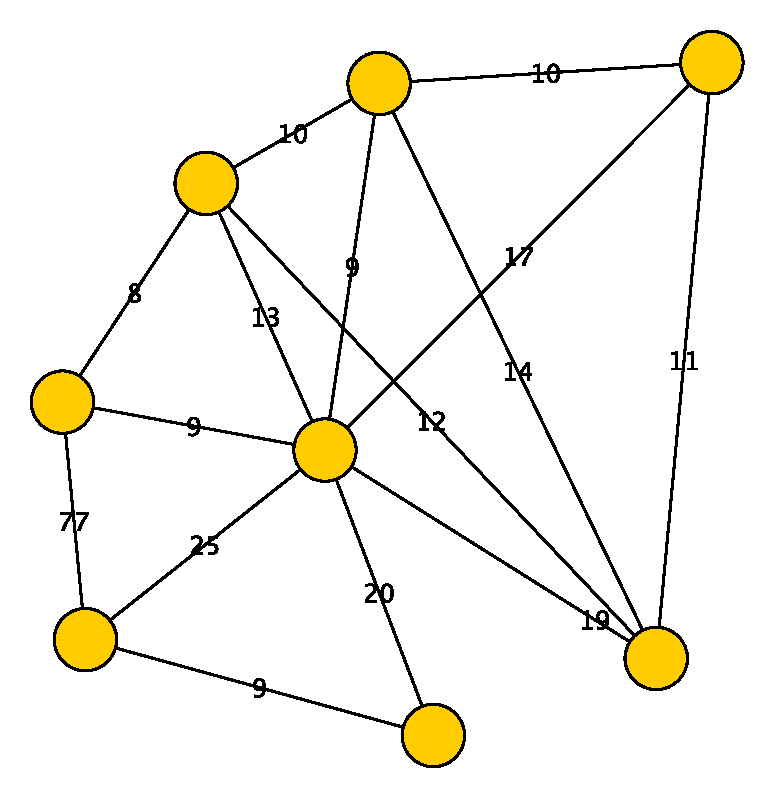
\includegraphics[width=0.7\linewidth]{shortestpath}
			\end{center}
		\newpage
		\item Suppose AJ wants to do a secured take home exam. He came up with the following scheme. He first list out the list of students and find out who is friend with whom. If they are friend and AJ give out the same version of the exam to both there is a chance that they will copy each other. AJ could give out different exam for everyone but that would interfere with AJ gaming schedule too much. Use something you learn from graph theory to figure out the number of minimum different version exam paper he needs to make. (1 means friend 0 means not friend)
		
		\begin{center}
			\begin{tabular}{|c|c|c|c|c|c|c|c|c|}
				\hline
				 & A & B & C & D & E & F & G & H\\
				 \hline
				 A & - & 0 & 1 & 1 & 0 & 1 & 1 & 0\\
				 B & - & - & 0 & 0 & 0 & 0 & 1 & 1\\
				 C & - & - & - & 1 & 1 & 1 & 0 & 1\\
				 D & - & - & - & - & 0 & 1 & 0 & 0\\
				 E & - & - & - & - & - & 0 & 1 & 1\\
				 F & - & - & - & - & - & - & 1 & 1\\
				 G & - & - & - & - & - & - & - & 1\\
				 H & - & - & - & - & - & - & - & -\\
				\hline
			\end{tabular} 
		\end{center}
		\manswer
		
		\item Find an isomorphism between these two graphs.	
		\begin{center}
		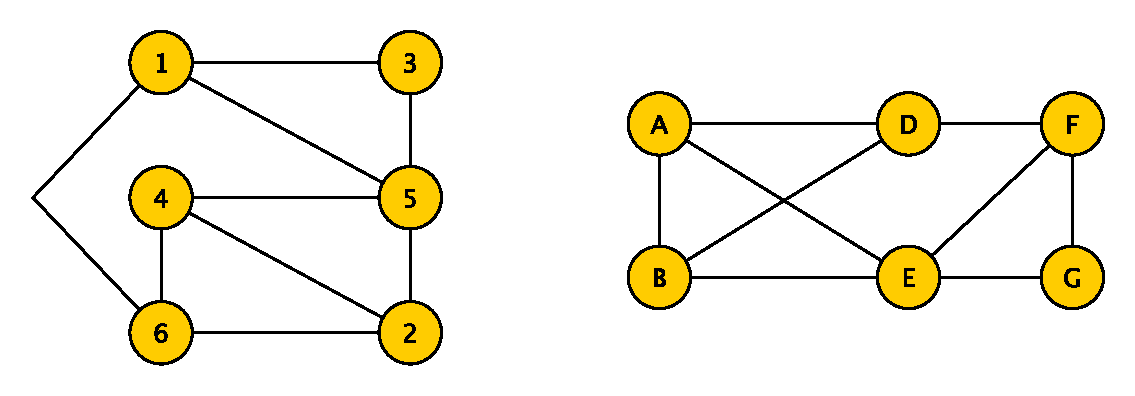
\includegraphics[width=0.7\linewidth]{isomorphism1}
		\end{center}
		
	\end{enumerate}
		
	\newpage 
	\item (20 each) Consider a popular ramen stall. Before the shop opens, there are 20 people waiting in front of the restaurant. (Make sure to write a short description for each term.)
	\begin{enumerate}
		\item How many ways are there to form a single line from these 20 people?
		\sanswer
		\item How many ways are there to form two \textbf{equal} lines(order matters) from 20 people? (The two lines are indistinguishable).
		\sanswer
		\item How many ways are there to form two \emph{indistinguishable} lines from 20 people? Each line may contain from 0 to 20 people but the total must add up to 20 and the order of people in each line matters.
		\sanswer
		\item The ramen shop only serve 10 bowls a day. The shop owner pick only 10 from 20 people and kick the rest out. How many combinations of people who gets to eat are there? (Order doesn't matter)
		\sanswer
		\item The ramen shop has only 2 menus: Shoyu Ramen and Seafood Ramen. Given that the shop only serves 10 bowls per day. If each person can only order exactly one bowl from the menu, how many combination of ramen orders(how each customer order) are there? (Each customer is distinguishable.)
		\sanswer
		\newpage
		\item Given that the shop only serves 10 bowls per day. If the maximum number of each menu the customers can order is 7 which means if the first 7 people order Shoyu Ramen, the rest must order Seafood Ramen. How many combination of ramen orders(how each customer order and who got kicked out) are there?
		
		Ex: People can still order 5 Shoyu and 5 Seafood if they wish.
		But, no, the 10 people who gets in can't order 8 Shoyu and 2 Seafood.
		
		\sanswer
	\end{enumerate}
		
	\newpage
	
	\item (20 each)
	
	Each medical test has pro and cons. Extremely specific(very few false positive) medical test is typically very expensive while a less accurate one costs less. So typically what we do is to use less accurate and less expensive one as a screening test administered to wider population.
	
	In this problem, we are going to examine a two-step medical test for a disease that 20\% of the population have the disease. \textbf{First we screen the people using less expensive test and for those whose test come out positive we are going to get them to a more expensive test. If the first test says no, then no more test is required. The person is confirmed positive if \emph{both} tests say yes.}
	
	Here are the information about the two tests.
	
	\subsection*{Screening Test}
		\begin{itemize}
			\item Costs 100 Baht per person
			\item Specification
			\begin{itemize}
				\item If you have the disease, there is a 90\% chance the test says yes.
				\item if you do not have the disease, there is a 30\% chance the test says yes.
			\end{itemize}
		\end{itemize}
		
	\subsection*{Expensive Test}
	\begin{itemize}
		\item The result is independent to screening test result.
		\item Costs 5000 Baht per person.
		\item Specification
		\begin{itemize}
			\item If you have the diesease there is a 95\%, chance the test says yes.
			\item If you do not have the disease, there is a 5\% chance the test says yes.
		\end{itemize}
	\end{itemize}
	
	\begin{enumerate}
	
	\item If you have the disease, what is the probability that you are confirmed postive.
	\sanswer
	\item If you do not have the disease what is the probability that you are confirmed positive.
	\manswer
	\item Given that you are confirmed positive what is the probability that you have the disease?
	\sanswer
	\item Given that you are \emph{not} confirmed positive what is the probability that you \emph{do not} have the disease?
	\sanswer
	\item If you have the diesase, what is the amount of money you are expected to pay as testing fee?
	\sanswer
	\item If you have the disease what is the \emph{variance} of total medical test fee?
	\sanswer
	\item If you do not have the diesease what is the amount of money you are expected to pay as testing fee?
	\sanswer
	\item If we switch the two tests, that is to have people go through expensive test first then cheaper one. Find the new false negative rate. (False negative is the probability that you have the disease but the process says no.)
	\sanswer
	\end{enumerate}

	%Linearity of Expected Value

	
%	%Expected Value and Variance Property


	\newpage
	\item (20 each) Consider two lottery players(Appy and Gordon) with different strategies. The lottery itself has number from 00-99 (total of 100 numbers). One winning number is selected randomly from that 100 numbers. Each lottery cost 80 Baht and if it's the winning number then the buyer with that number wins 2,000 Baht. (This is the actual number for Thai lotto)
	\begin{itemize}
		\item Appy buys 50 numbers independently and the numbers are selected from uniform probability. Yes, he may have some duplicates.
		\item Gordon buys 50 lotteries of exact same number.
	\end{itemize}
	\begin{enumerate}
		\item Find expected value of Gordon profit/loss (Winning Amount - Cost).
		\sanswer
		\item Find expected value of Appy profit/loss.
		\sanswer
		\item Find the standard deviation of Gordon's profit/loss.
		\sanswer
		\item Find the standard deviation of Appy profit/loss.
		\sanswer
		\item What is the probability that Appy will buy all 50 lotteries of the same number \textbf{and} that number happens to win?
		\manswer
		\item What is the probability that Gordon will make profit?
		\sanswer
		\item What is the probability that Appy will make profit? (You may need to think outside the box for this one.)
		\sanswer
	\end{enumerate}


\end{enumerate}


\end{document}